\par 
Die Umwelt wird in den allermeisten Fällen als Markow-Entscheidungsprozess (\textit{Markov Decision Process, MDP}) definiert. //TODO Als \textit{MDP} versteht sich die Formalisierung von sequentiellen Entscheidungsproblemen, bei denen eine Entscheidung nicht nur die sofortige Belohnung beeinflusst, sondern auch alle Folgezustände und somit auch alle zukünftigen Belohnungen (S. 47). Zudem bieten sie den mathematischen Rahmen für das \textit{Reinforcement Learning} Problem, um z.B. Beweise über das Konvergenzverhalten eines Algorithmus hin zu einer optimalen Strategie führen oder andere theoretische Aussagen treffen zu können. Außerdem müssen Probleme die als \textit{MDP} definiert werden zugleich die Markow-Eigenschaft erfüllen, die von essentieller Bedeutung ist und in Kapitel X näher erläutert wird.
\par 

\begin{figure}[H]
    \centering
    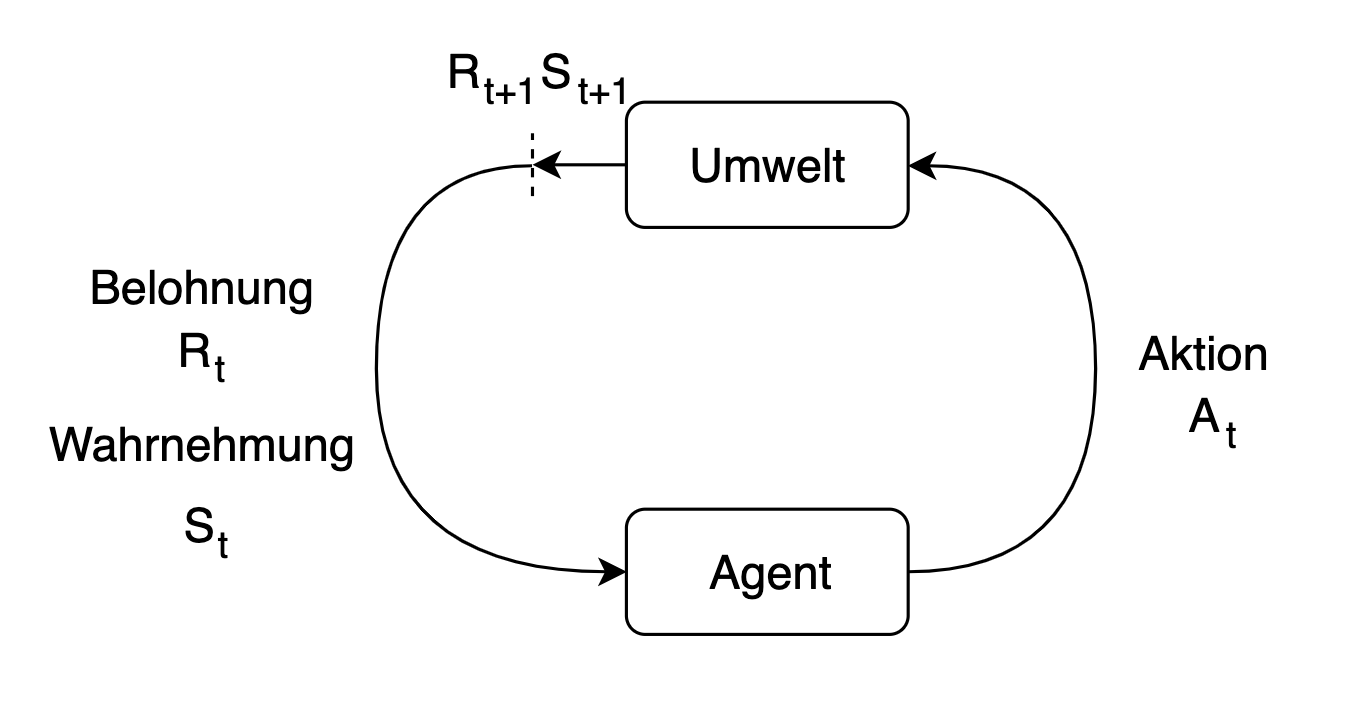
\includegraphics[height=150px]{images/agentUmweltInterface.png}
    \caption{Agent-Umwelt Interface}
\end{figure}


Der Agent interagiert mit dem \textit{MDP} jeweils zu diskreten Zeitpunkten $t = 0, 1, 2, 3, \dots$. \\
Zu jedem Zeitpunkt $t$ beobachtet der Agent den Zustand seiner Umgebung $S_t \in \mathcal{S}$ und wählt aufgrund dessen eine Aktionen $A_t \in \mathcal{A}$. Als Konsequenz seiner Aktion erhält er einen Zeitpunkt später eine Belohnung $R_{t+1} \in \mathcal{R} \subset\mathbb{R} $ und stellt den Folgezustand $S_{t+1}$ fest. Das Zusammenspiel zwischen Agenten und MDP erzeugt also folgende Reihenfolge:
\[S_0, A_0, R_1, S_1, A_1, R_2, S_2, A_2, R_3, \dots\]

Wird einfach nur von \textit{MDPs} gesprochen, ist die endliche Variante (\textit{finite MDP}) gemeint, bei dem die Mengen der Zustände, Aktionen und Belohnungen ($\mathcal{S}, \mathcal{A}, \mathcal{R}$) eine endliche Anzahl an Elementen besitzen. In diesem Fall haben die zufälligen Variablen $R_t$ und $S_t$ wohl definierte diskrete Wahrscheinlichkeitsverteilungen, die nur von dem vorigen Zustand und vorigen Aktion abhängig sind (S.48). Die Wahrscheinlichkeit, dass die bestimmten Werte für diese Variablen $s' \in \mathcal{S}$ und $r \in \mathcal{R}$ eintreten, für einen bestimmten Zeitpunkt $t$ und dem vorigen Zustand $s$ und Aktion $a$, kann somit durch folgende Funktion beschrieben werden:

\[p(s',r \mid s,a) \doteq Pr\{S_t=s',R_t=r|S_{t-1}=s,A_{t_1}=a\},\]

für alle $s', s \in \mathcal{S}, r \in \mathcal{R}$ und $a \in \mathcal{A}(s)$. Diese Funktion p definiert die sog. Dynamiken (\textit{Dynamics}) eines \textit{MDP}. Sie ist eine gewöhnliche deterministische Funktion mit vier Parametern $p: \mathcal{S} \times \mathcal{R} \times \mathcal{A} \rightarrow [0,1]$. Das \glqq$\mid$\grqq{} Zeichen kommt ursprünglich aus der Notation für bedingte Wahrscheinlichkeiten, soll hier aber nur andeuten, dass es sich um eine Wahrscheinlichkeitsverteilung handelt für jeweils alle Kombinationen von $s$ und $a$:

\[ \sum_{s' \in \mathcal{S}} \sum_{r \in \mathcal{R}} p(s', r \mid s,a) = 1 \ \forall s \in \mathcal{S}, a \in \mathcal{A}(s)\]

Ist die Zustandsüberführungsfunktion nicht stochastisch, so ist $p$ immer nur für ein bestimmtes Triplet $(s,a,r)$ für jedes $s' \in \mathcal{S}$ gleich 1, für alle andere jeweils 0. Mit anderen Worten, wird im Zustand $s$ die Aktion $a$ gewählt, führt dies immer zu einem bestimmten Folgezustand $s’$. 
\par 

Das MDP Framework gilt als extrem flexibel und kann auf die unterschiedlichsten Probleme angewendet werden. Es bietet die nötige Abstraktion für Probleme, bei denen unter Vorgabe eines Ziels mittels Interaktionen gelernt wird. Dabei sind die Einzelheiten über eigentliche Ziel, die Zustände oder die Form des Agenten unerheblich, denn jedes zielgerichtete Lernen kann auf drei Signale reduziert werden, die zwischen dem Agenten und der Umwelt ausgetauscht werden. Ein Signal repräsentiert die Entscheidung, die der Agent getroffen hat (die Aktion), ein Signal repräsentiert die Basis, auf der er diese Entscheidung getroffen hat (der Zustand) und ein Signal definiert das zu erreichende Ziel (die Belohnung).

